\begin{frame}{注意力机制}
\begin{itemize}
\item 注意力机制:Ours vs. TLLT\footnote[frame]{\tiny C. Gong et al. Saliency propagation from simple to difficult. CVPR 2015.}
\begin{figure}
    \centering
    \includegraphics[width=.5\linewidth]{figures/TLLT.png}
\end{figure}
\end{itemize}

\end{frame}

%%%
\begin{frame}{方法对比:Ours vs. Unet}
\begin{columns}[c]
\column{.6\textwidth}
\begin{table}
  \caption{实验结果(Vit2019)}
    \begin{tabular}{c|c|c}
    \toprule
   方法 & 监督方式 & mIoU \\
    \hline
    \hline
    FCN-VGG16  & \multirow{2}[2]{*}{Fully} & 72.4 \\
    U-net &       & 78.6 \\
    \hline
    PRM  & \multirow{3}[2]{*}{Weakly} & 67.2 \\
    SEC  &       & 64.7 \\
    Our Method &       &\textbf{71.4}\\
    \bottomrule
    \end{tabular}%
\end{table}%

\column{.5\textwidth}
\begin{figure}
    \centering
    \includegraphics[width=\linewidth]{figures/unetcompareSmaller.png}
\end{figure}
\end{columns}
\end{frame}

%%%
\begin{frame}{方法对比:Ours vs. SEC,PRM}
\begin{figure}
    \centering
    \includegraphics[width=.95\linewidth]{figures/weaklySupervisedCompare.png}
    \vspace{-.5em}
    \caption{弱监督方法效果对比:Ours vs. SEC\footnote[frame]{\tiny A. Kolesnikov and C. H. Lampert. Seed, Expand and Constrain:
Three Principles for Weakly-Supervised Image Segmentation. arXiv.org, Mar. 2016.},PRM\footnote[frame]{\tiny Y. Zhou et al. Weakly Supervised Instance Segmentation using Class Peak Response. arXiv.org, Apr. 2018.}}
\end{figure}
\end{frame}
%%%
\begin{frame}{显著图质量分析}
\begin{columns}[c]
\column{.4\textwidth}
\begin{figure}
    \centering
    \includegraphics[width=\linewidth]{figures/slaiencyquality.png}
\end{figure}

\column{.6\textwidth}
\begin{figure}
    \centering
    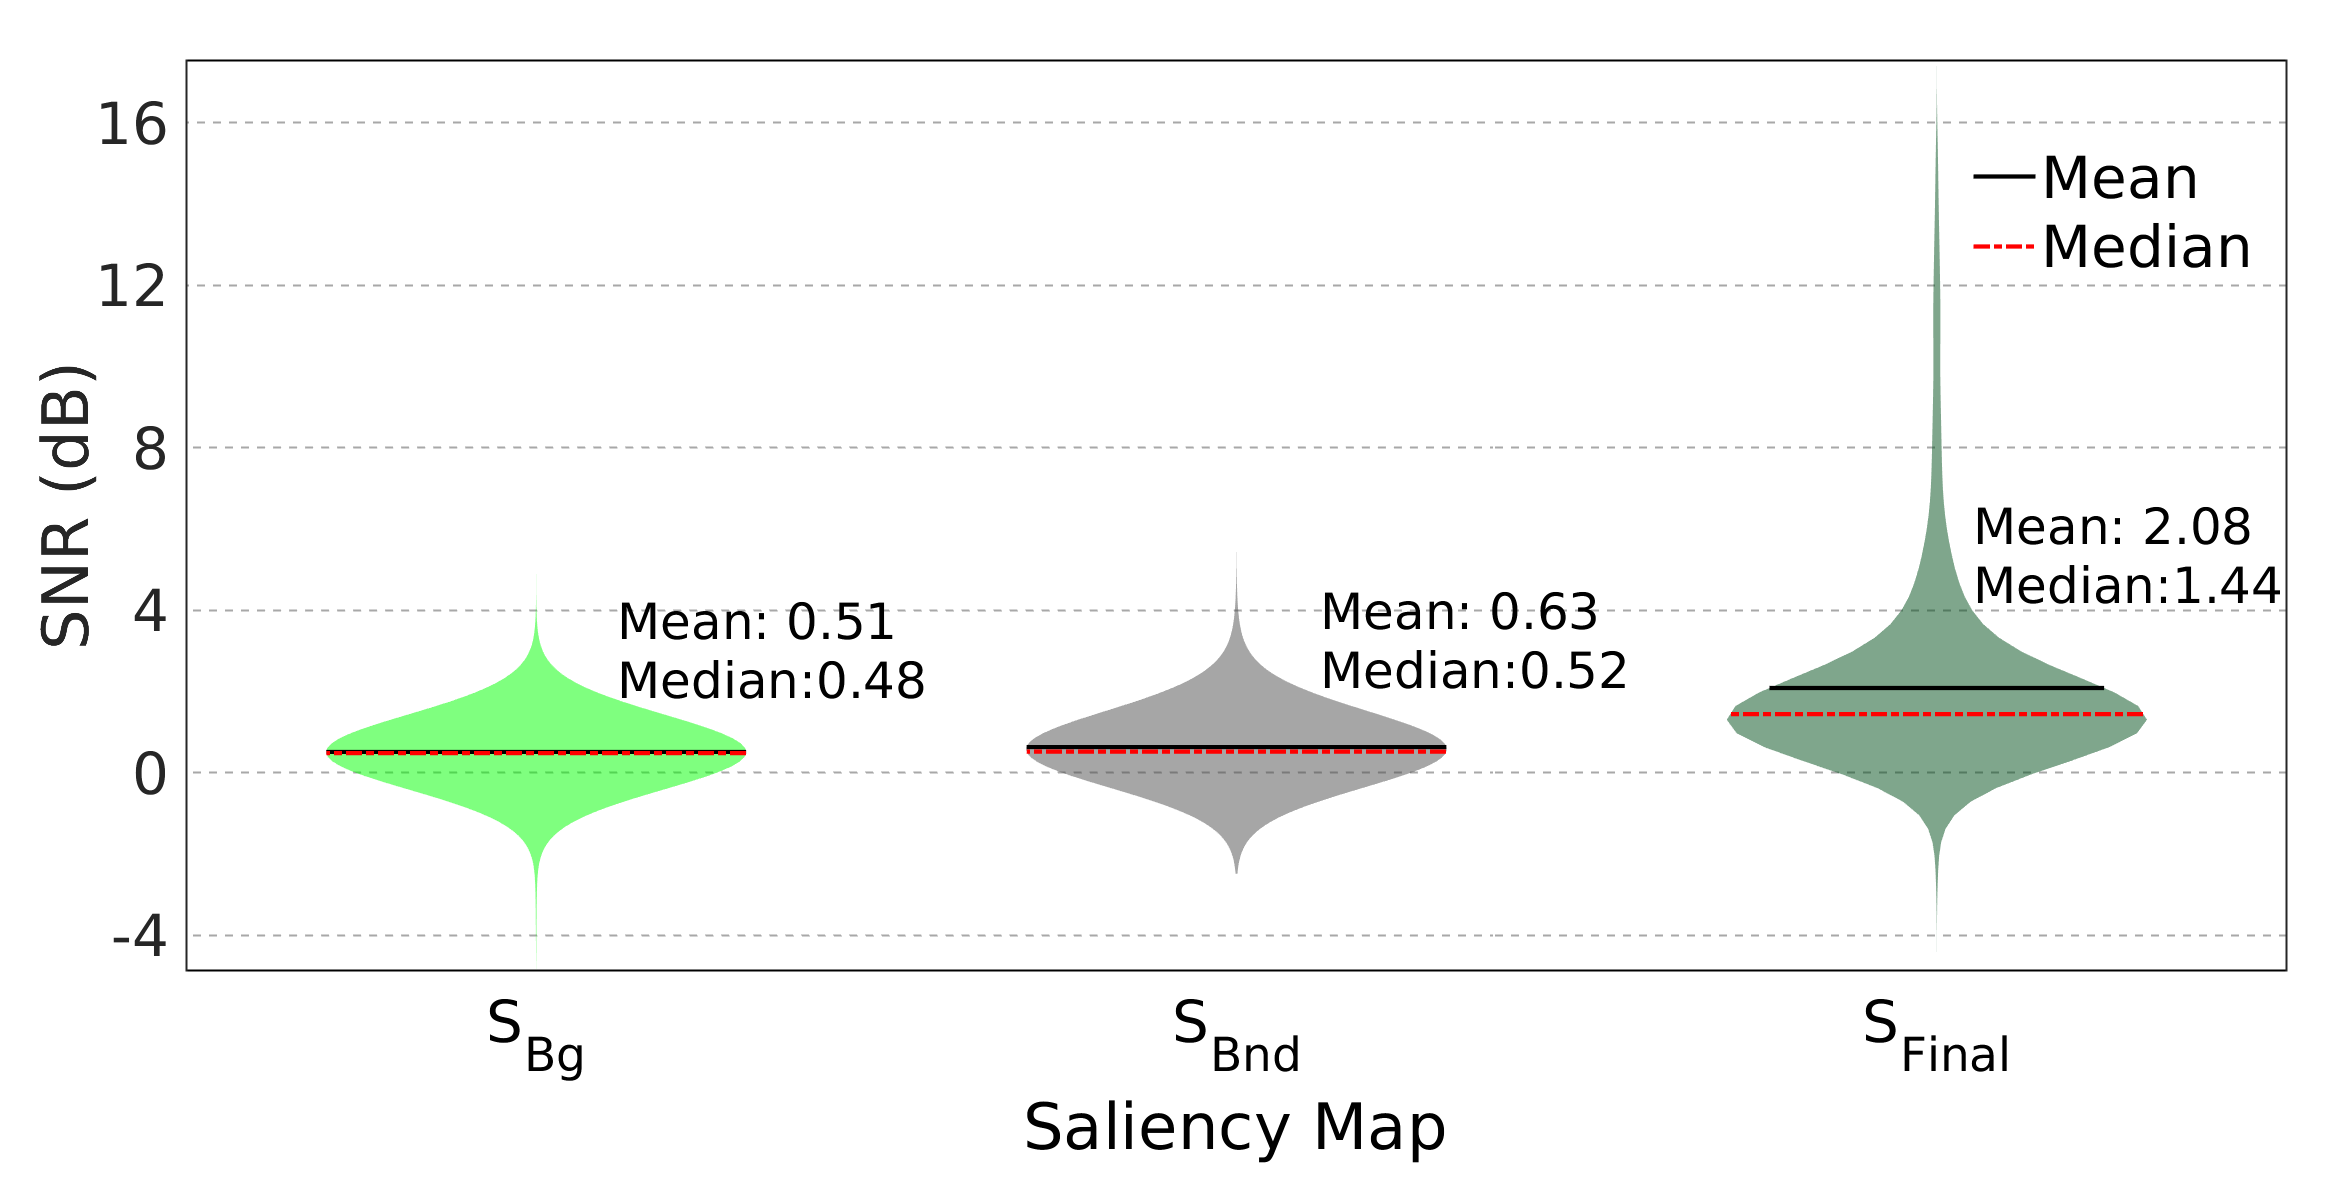
\includegraphics[width=\linewidth]{figures/VitViolin.eps}
\end{figure}

\vspace{-.4cm}

\begin{block}{定义}\small
信号:皮损区域内的显著性值

噪声:皮损区域外的显著性值
\end{block}

\vspace{-.2cm}

\begin{equation}\small
\mathrm{SNR_{dB}}=10\mathrm{log_{10}}(\frac{E_{\mathrm{signal}}}{E_{\mathrm{noise}}}) \nonumber
\end{equation}
\end{columns}
\end{frame}
%%%
\begin{frame}{Ablation Study}
\begin{figure}
    \centering
    \includegraphics[width=0.9\linewidth]{figures/CNNandSuperPixelModelGraph3.jpg}
\end{figure}
\vfill
\begin{table}[]
\label{tab:ablation}
\begin{center}
\setlength{\tabcolsep}{1 mm}{
    \begin{tabular}{c|cccccccc}
    \toprule
    Fg Mask & \xmark &   \cmark    &    \cmark   &   \cmark    & \xmark & \xmark & \xmark & \cmark \\
    Bg Seeds &  \cmark     & \xmark &   \cmark    & \xmark &  \cmark     & \xmark &  \cmark     & \cmark \\
    Bnd Seeds &  \cmark     &   \cmark    & \xmark & \xmark & \xmark &   \cmark    &   \cmark    & \cmark \\
    Last SP &   \cmark    &   \cmark    & \cmark      &   \cmark    &  \cmark     &    \cmark   &\xmark & \cmark \\
    \midrule
    IoU  & 62.5  & 66.7  & 63.1  & 59.5  & 43.5  & 53.0  & 57.7  & \textbf{71.4}  \\
    \bottomrule
    \end{tabular}}%
\end{center}
\end{table}%
\end{frame}
%%%
\begin{frame}{敏感度测试}
\begin{figure}
    \centering
    \includegraphics[width=0.8\linewidth]{figures/composit1.eps}
\end{figure}
\end{frame}








